\documentclass[10pt,a4paper]{article}
\usepackage[utf8]{inputenc}
\usepackage{graphicx}
\def\Pr{\mathop{\rm Pr}}
%\usepackage[landscape,margin=1cm]{geometry}
\usepackage[english]{babel}
\usepackage{tikz}
\usetikzlibrary{arrows,snakes,backgrounds,shapes.geometric}

%\date{July 2019}
\usepackage[default]{raleway}
\usepackage{fontawesome}
\usepackage[T1]{fontenc}

\usepackage{hyperref}
\usepackage{enumitem}
\usepackage{lipsum}

\usepackage{xcolor}
\definecolor{customcolor}{HTML}{616AC5}
\definecolor{alert}{HTML}{CD5C5C}
\definecolor{w3schools}{HTML}{4CAF50}
\definecolor{subbox}{gray}{0.60}
\definecolor{codecolor}{HTML}{FFC300}
\colorlet{xx}{customcolor}


%--------------------------Editor mode.

\usepackage
[citestyle=authoryear,
sorting=nty,	  		%Sorts bibliography by year, name, title
autocite=footnote, 		%Autocite command generates footnotes
autolang=hyphen, 		
mincrossrefs=1, 	
backend=biber]
{biblatex}

\DeclareFieldFormat{postnote}{#1}
\DeclareFieldFormat{multipostnote}{#1}
\DeclareAutoCiteCommand{footnote}[f]{\footcite}{\footcites}

\bibliography{literature}
%----------------------------------------
%--------------------------------------------------------------------------------
\usepackage{tcolorbox}

\tcbuselibrary{most,listingsutf8,minted}

\tcbset{tcbox width=auto,left=1mm,top=1mm,bottom=1mm,
right=1mm,boxsep=1mm,middle=1pt}

\newenvironment{mycolorbox}[2]{%
\begin{tcolorbox}[grow to left by=-1em,grow to right by=-1em,capture=minipage,fonttitle=\large\bfseries, enhanced jigsaw,boxsep=1mm,colback=#1!30!white,on line,tcbox width=auto, toptitle=0mm,colframe=#1,opacityback=0.7,nobeforeafter,title=#2]%
}{\end{tcolorbox}\\[0.2em]}

\newenvironment{subbox}[2]{%
\begin{tcolorbox}[capture=minipage,fonttitle=\normalsize\bfseries, enhanced jigsaw,boxsep=1mm,colback=#1!30!white,on line,tcbox width=auto,left=0.3em,top=1mm, toptitle=0mm,colframe=#1,opacityback=0.7,nobeforeafter,title=#2]\footnotesize %
}{\normalsize\end{tcolorbox}\vspace{0.1em}}

\newenvironment{multibox}[1]{%
\begin{tcbraster}[raster columns=#1,raster equal height,nobeforeafter,raster column skip=1em,raster left skip=1em,raster right skip=1em]}{\end{tcbraster}}

\newenvironment{textbox}[1]{\begin{mycolorbox}{customcolor}{#1}}{\end{mycolorbox}}

%-------------------------------
\newtcblisting{codebox}[2]{colback=codecolor!5,colframe=codecolor!80!black,listing only, 
minted options={numbers=left,style=tcblatex,fontsize=\tiny,breaklines,autogobble,linenos,numbersep=1mm},
left=5mm,enhanced,
title=#2, fonttitle=\bfseries,
listing engine=minted,minted language=#1}

%--------------------------------------------------------------------------------
\newcommand{\punkti}{~\lbrack\dots\rbrack~}

\renewenvironment{quote}
               {\list{\faQuoteLeft\phantom{ }}{\rightmargin\leftmargin}%
                \item\relax\scriptsize\ignorespaces}
               {\unskip\unskip\phantom{xx}\faQuoteRight\endlist}
               

%--------------------------------------------------------------------------------
\newcommand{\bgupper}[3]{\colorbox{#1}{\color{#2}\huge\bfseries\MakeUppercase{#3}}}
\newcommand{\bg}[3]{\colorbox{#1}{\bfseries\color{#2}#3}}

\newcommand{\mycommand}[2]{{\ttfamily\detokenize{#1}}~\dotfill{}~{\footnotesize #2}\\}
\newcommand{\sep}{{\scriptsize~\faCircle{ }~}}


\newcommand{\bggreen}[1]{\medskip\bgupper{w3schools}{black}{#1}\\[0.5em]}
\newcommand{\green}[1]{\smallskip\bg{w3schools}{white}{#1}\\}
\newcommand{\red}[1]{\smallskip\bg{alert}{white}{#1}\\}

\usepackage{multicol}
\setlength{\columnsep}{30pt}

\setlength{\parindent}{0pt}
\pagestyle{empty}

\usepackage{csquotes}

\newcommand{\loremipsum}{Lorem ipsum dolor sit amet.}


%--------------------------------------------------------------------------------
\begin{document}

%\maketitle
%\thispagestyle{empty}
\scriptsize
%\tableofcontents


\begin{textbox}{Flowchart }
\begin{subbox}{subbox}{ Double Loop}
\begin{center}
    
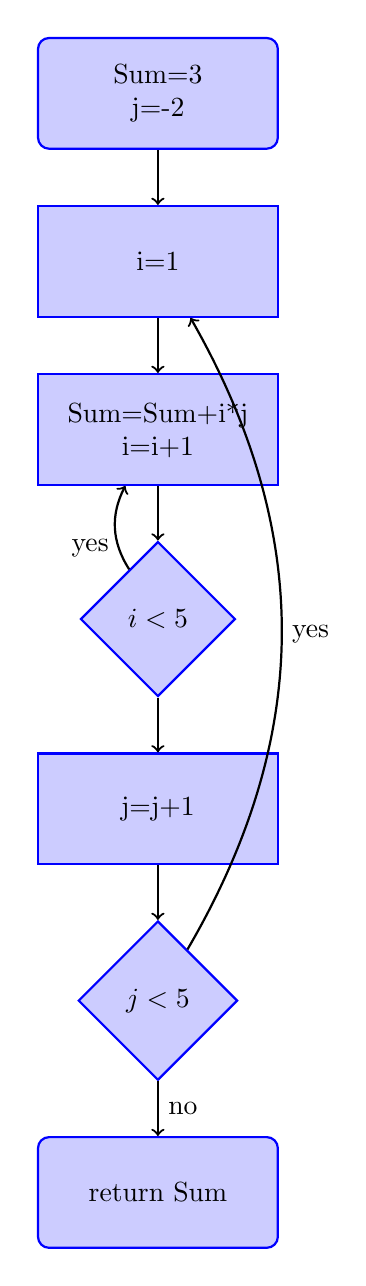
\begin{tikzpicture}[auto]
\tikzstyle{decision} = [diamond, draw=blue, thick, fill=blue!20,
text width=4.5em, text badly centered, inner sep=1pt]

\tikzstyle{block} = [rectangle, draw=blue, thick, fill=blue!20,
text width=8em, text centered, rounded corners, minimum height=4em]
\tikzstyle{block_op} = [rectangle, draw=blue, thick, fill=blue!20,
text width=8em, text centered, minimum height=4em]
\tikzstyle{line} = [draw, thick,->];
\tikzstyle{cloud} = [draw=red, thick, ellipse,fill=red!20, minimum height=2em];
\matrix [column sep=5mm,row sep=7mm]
{
% row 1
 \node [block] (init) { Sum=3\\j=-2}; & \\
% row 2
\node [block_op] (identify) {i=1}; & ;\\
% row 4
\node [block_op] (identify2) {Sum=Sum+i*j\\
i=i+1}; & ;\\
\node [decision] (decide) {$i<5$}; & \\
% row 5
\node [block_op] (identify3) {
j=j+1}; & ;\\
\node [decision] (decide2) {$j<5$}; & \\
\node [block] (stop) {return Sum}; & \\
};
\tikzstyle{every path}=[line]
\path (init) -- (identify);
\path (identify) -- (identify2);
%\path (identify) -- (decide);
%\path (decide)  edge [bend right] node[near start,right] {yes}  (identify);
%\path (decide) -- node [midway] {no} (identify2);
\path (identify2) -- (decide);
\path (decide) -- (identify3);

\path (identify3) -- (decide2);
%\path (decide2) -- (stop);

\path (decide2)  edge [bend right] node[right] {yes}  (identify);

\path (decide)  edge [bend left] node[near start,left] {yes}  (identify2);

\path (decide2) -- node [midway] {no} (stop);

\end{tikzpicture}

\end{center}
\end{subbox}

\end{textbox}
%%%%%% Q1b
\newpage
\begin{textbox}{Flowchart }
\begin{subbox}{subbox}{Arithmetic Series}
\begin{center}
    
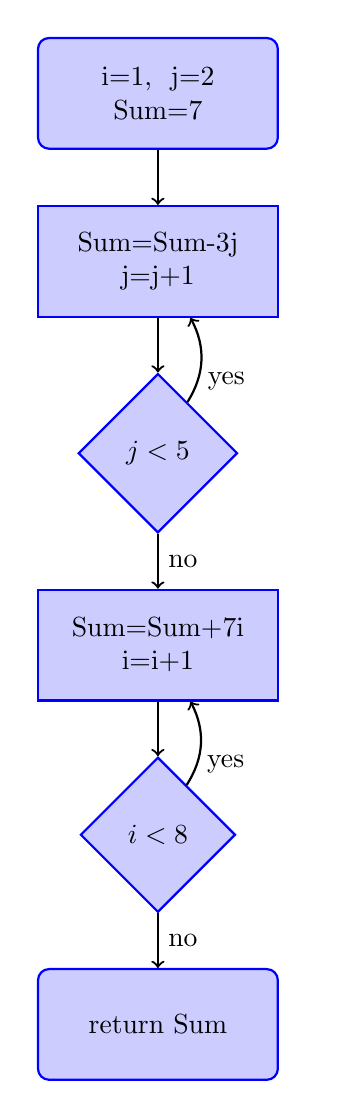
\begin{tikzpicture}[auto]
\tikzstyle{decision} = [diamond, draw=blue, thick, fill=blue!20,
text width=4.5em, text badly centered, inner sep=1pt]

\tikzstyle{block} = [rectangle, draw=blue, thick, fill=blue!20,
text width=8em, text centered, rounded corners, minimum height=4em]
\tikzstyle{block_op} = [rectangle, draw=blue, thick, fill=blue!20,
text width=8em, text centered, minimum height=4em]
\tikzstyle{line} = [draw, thick,->];
\tikzstyle{cloud} = [draw=red, thick, ellipse,fill=red!20, minimum height=2em];
\matrix [column sep=5mm,row sep=7mm]
{
% row 1
 \node [block] (init) {i=1, \ j=2\\ Sum=7\\}; & \\
% row 2
\node [block_op] (identify) {
Sum=Sum-3j\\
j=j+1}; & ;\\
% row 4
\node [decision] (decide) {$j<5$}; & \\
% row 5
\node [block_op] (identify_i) {
Sum=Sum+7i\\
i=i+1}; & ;\\
\node [decision] (decide_i) {$i<8$}; & \\
% row 5
\node [block] (stop) {return Sum}; & \\
};
\tikzstyle{every path}=[line]
\path (init) -- (identify);
\path (identify) -- (decide);
\path (decide)  edge [bend right] node[near start,right] {yes}  (identify);
\path (decide) -- node [midway] {no} (identify_i);
\path (identify_i) -- (decide_i);
\path (decide_i)  edge [bend right] node[near start,right] {yes}  (identify_i);
\path (decide_i) -- node [midway] {no} (stop);
\end{tikzpicture}

\end{center}
\end{subbox}
\end{textbox}



%%%%%% Q1c
\newpage
\begin{textbox}{Flowchart }
\begin{subbox}{subbox}{Arithmetic Series}
\begin{center}
    
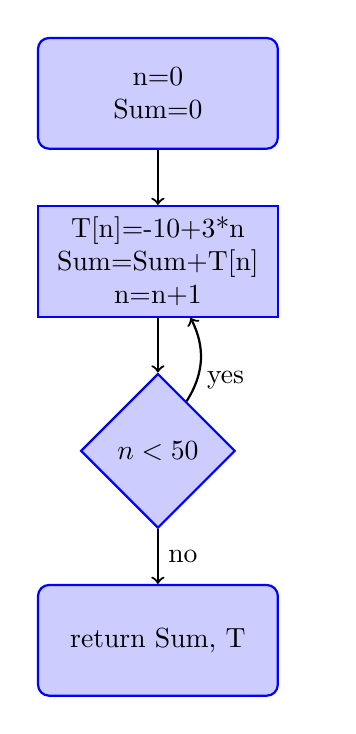
\begin{tikzpicture}[auto]
\tikzstyle{decision} = [diamond, draw=blue, thick, fill=blue!20,
text width=4.5em, text badly centered, inner sep=1pt]

\tikzstyle{block} = [rectangle, draw=blue, thick, fill=blue!20,
text width=8em, text centered, rounded corners, minimum height=4em]
\tikzstyle{block_op} = [rectangle, draw=blue, thick, fill=blue!20,
text width=8em, text centered, minimum height=4em]
\tikzstyle{line} = [draw, thick,->];
\tikzstyle{cloud} = [draw=red, thick, ellipse,fill=red!20, minimum height=2em];
\matrix [column sep=5mm,row sep=7mm]
{
% row 1
 \node [block] (init) {n=0 \\ Sum=0}; & \\
% row 2
\node [block_op] (identify) {T[n]=-10+3*n\\
Sum=Sum+T[n]\\
n=n+1}; & ;\\
% row 4
\node [decision] (decide) {$n<50$}; & \\
% row 5
\node [block] (stop) {return Sum, T}; & \\
};
\tikzstyle{every path}=[line]
\path (init) -- (identify);
\path (identify) -- (decide);
\path (decide)  edge [bend right] node[near start,right] {yes}  (identify);
\path (decide) -- node [midway] {no} (stop);

\end{tikzpicture}

\end{center}
\end{subbox}
\end{textbox}

%%%%%% Q1d
\newpage
\begin{textbox}{Flowchart }
\begin{subbox}{subbox}{Approx $e^{-2x}$}
\begin{center}
    
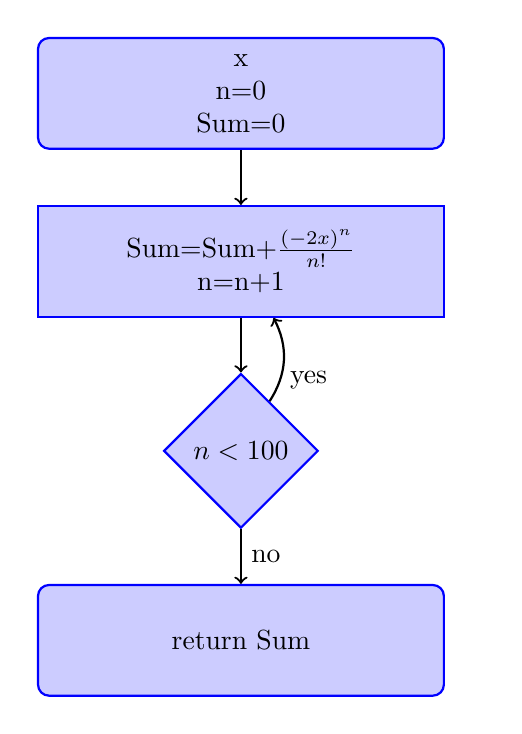
\begin{tikzpicture}[auto]
\tikzstyle{decision} = [diamond, draw=blue, thick, fill=blue!20,
text width=4.5em, text badly centered, inner sep=1pt]

\tikzstyle{block} = [rectangle, draw=blue, thick, fill=blue!20,
text width=14em, text centered, rounded corners, minimum height=4em]
\tikzstyle{block_op} = [rectangle, draw=blue, thick, fill=blue!20,
text width=14em, text centered, minimum height=4em]
\tikzstyle{line} = [draw, thick,->];
\tikzstyle{cloud} = [draw=red, thick, ellipse,fill=red!20, minimum height=2em];
\matrix [column sep=5mm,row sep=7mm]
{
% row 1
 \node [block] (init) {x\\n=0 \\ Sum=0}; & \\
% row 2
\node [block_op] (identify) {
Sum=Sum+$\frac{(-2x)^n}{n!}$\\
n=n+1}; & ;\\
% row 4
\node [decision] (decide) {$n<100$}; & \\
% row 5
\node [block] (stop) {return Sum}; & \\
};
\tikzstyle{every path}=[line]
\path (init) -- (identify);
\path (identify) -- (decide);
\path (decide)  edge [bend right] node[near start,right] {yes}  (identify);
\path (decide) -- node [midway] {no} (stop);

\end{tikzpicture}

\end{center}
\end{subbox}
\end{textbox}
\end{document}
